\begin{frame}{Linear Models for Regression}
    \begin{figure}
    \centering
    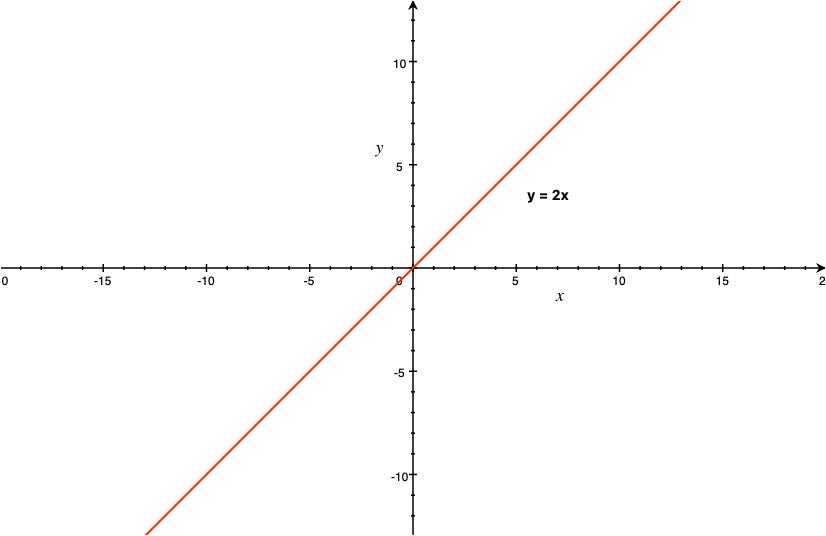
\includegraphics[width=.7\textwidth]{img/line.jpg}
    \caption{$y$ is given as a function of $x$ in the form $y=mx+b$}
    \end{figure}
\end{frame}

\begin{frame}{Linear Models for Regression}
\begin{itemize}
    \item Data is a collection of paired points such as
    $$(0, 0), (1, 1), (2.5, 2), (5, 6), ...$$
    \item We assume data can be fit by a linear hypothesis function
    $$y = w_1x + b$$
    \item \textbf{Our job:} Given just this data, how to choose $w_1$ and $b$?
\end{itemize}
\end{frame}

\begin{frame}{Linear Models for Regression}
\begin{figure}
    \centering
    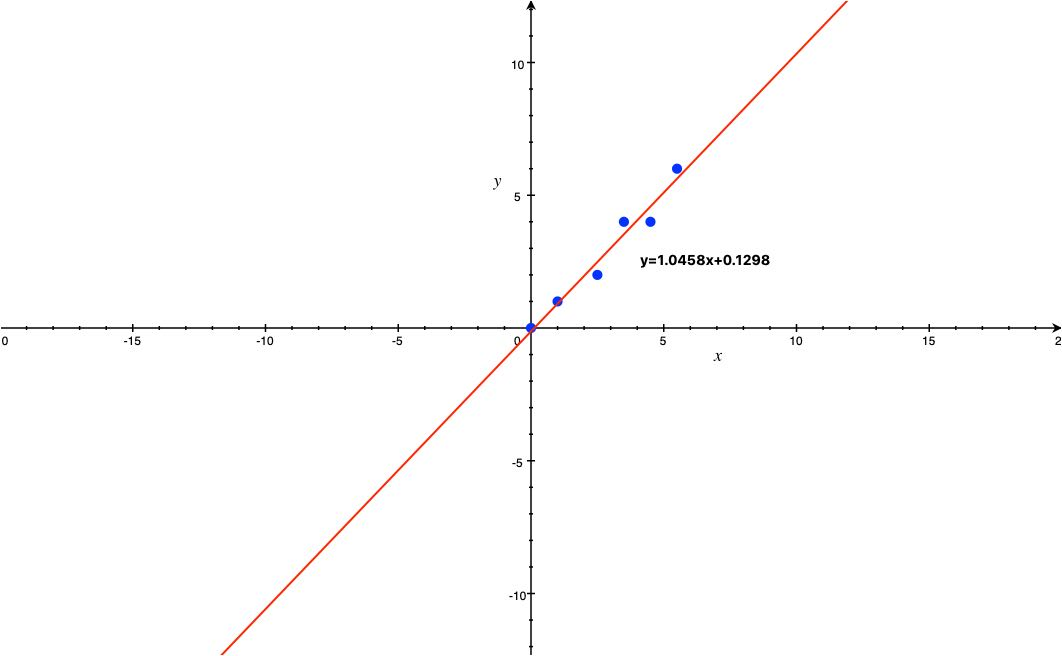
\includegraphics[width=.7\textwidth]{img/regressed_points.jpg}
    \caption{Line interpolated for 2D blue point dataset}
\end{figure}
\end{frame}

\begin{frame}{Linear Models for Regression}
\begin{itemize}
    \item First, we generalize the problem statement a little bit...
    \item You can have more than just one feature $x$.
    \item Instead of just using $ft^2$ to predict price of house, you also include which city your house is in because apartment in San Francisco is small but expensive!
    \item Data of any number of $x$ can be fit by a linear hypothesis function 
    $$y = w_0 + w_1x_1 + ... + w_Dx_D$$
\end{itemize}
\end{frame}

\begin{frame}{Linear Models for Regression}
\begin{figure}
    \centering
    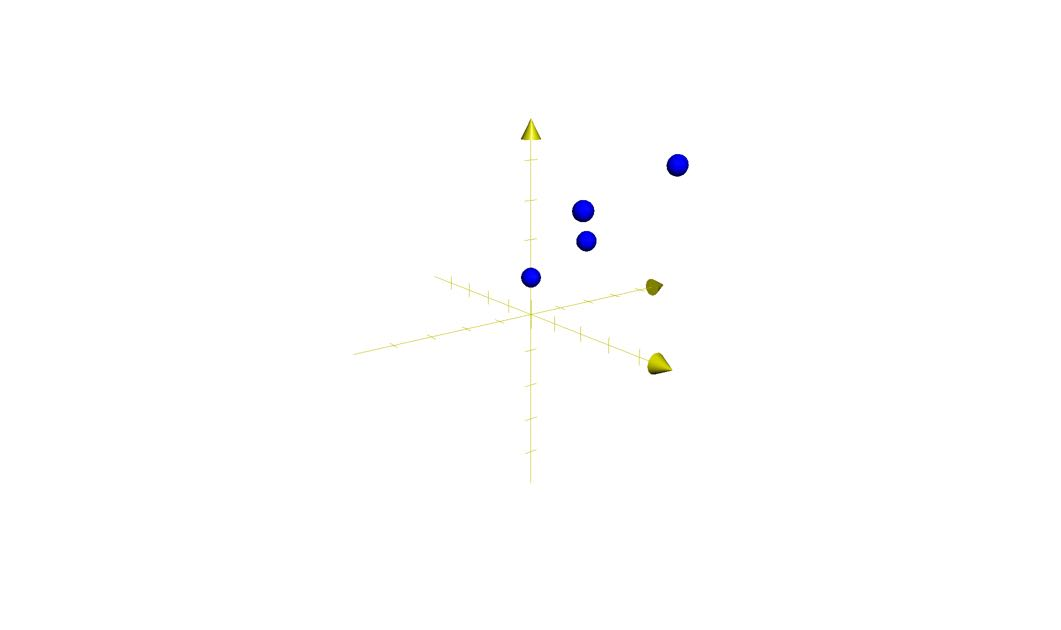
\includegraphics[width=0.9\textwidth]{img/3d_regressed_points.jpg}
    \caption{3D blue point dataset $(x_1, x_2, y)$}
\end{figure}
\end{frame}

\begin{frame}{Linear Models for Regression}
\begin{figure}
    \centering
    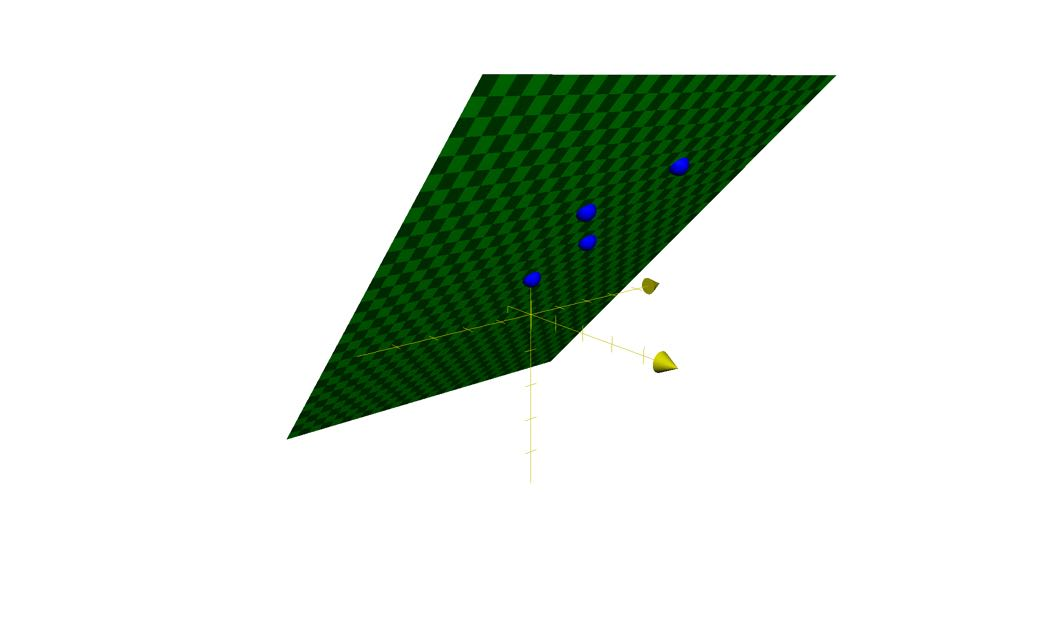
\includegraphics[width=0.9\textwidth]{img/3d_regressed_line.jpg}
    \caption{Regressed \textit{plane}: $y= x_1 - x_2 +1$}
\end{figure}
\end{frame}

\begin{frame}{Linear Models for Classification}
\begin{itemize}
    \item In the regression case, we take input $(x_1, x_2, ..., x_D)$ and return the point $y$ that fits our linear hypothesis function $$y = w_0 + w_1x_1 + ... + w_Dx_D$$ where
    $$y, x_1, x_2, ..., x_D \in \mathbb{R}$$
    \item The goal in classification is to take input $(x_1, x_2, ..., x_D)$ and assign it to one of $K$ groups.
    \item Example of K = 2?
\end{itemize}
\end{frame}

\begin{frame}{Linear Models for Classification}
\begin{itemize}
    \item In the regression case, we take input $(x_1, x_2, ..., x_D)$ and return the point $y$ that fits our linear hypothesis function $$y = w_0 + w_1x_1 + ... + w_Dx_D$$ where
    $$y, x_1, x_2, ..., x_D \in \mathbb{R}$$
    \item The goal in classification is to take input $(x_1, x_2, ..., x_D)$ and assign it to one of $K$ groups.
    \item Example of $K = 2$? 
    
    pass/fail, win/lose, healthy/sick, poor/not poor, hotdog/not hotdog,
    \item We will continue to focus on $K = 2$ case, known as \textbf{binary classification}.
\end{itemize}
\end{frame}

\begin{frame}{Linear Models for Classification}
\begin{itemize}
    \item Regression returns the "real" numeric value we want, e.g. house price in dollars.
    \item Less intuitive: How to capture "group assignment" numerically? 
\end{itemize}
\end{frame}

\begin{frame}{Linear Models for Classification}
\begin{itemize}
    \item Regression returns the "real" numeric value we want, e.g. house price in dollars.
    \item Less intuitive: How to capture "group assignment" numerically? 
    \item Classification models return the \textbf{probability} that input belongs to a group.
\end{itemize}
\end{frame}

\begin{frame}{Linear Models for Classification}
\begin{itemize}
    \item Regression returns the "real" numeric value we want, e.g. house price in dollars.
    \item Less intuitive: How to capture "group assignment" numerically? 
    \item Classification models return the \textbf{probability} that input belongs to a group.
    \item For binary classification: We need to find some function $f$ defined as $$p = f(x_1, x_2, ..., x_D)$$ that takes $(x_1, ..., x_D)$, does some math, and returns a probability $p$ of belonging to Group 1.
    \item Probability of being in Group 2 is given by $1-p$.
\end{itemize}
\end{frame}

\begin{frame}{Linear Models for Classification}
\begin{itemize}
    \item We use a modified version of our linear regression function:
    $$y = \sigma(w_0 + w_1x_1 + ... + w_Dx_D)$$
    \item Where $\sigma$ is the \textbf{sigmoid} function, a type of logistic funciton given by
    $$\frac{1}{1 + e^{-x}}$$
    \item In statistics, this model is known as \textbf{logistic regression}, although it should be emphasized that this is a model for classification rather than regression.
\end{itemize}
\end{frame}

\begin{frame}{Linear Models for Classification}
\begin{figure}
    \centering
    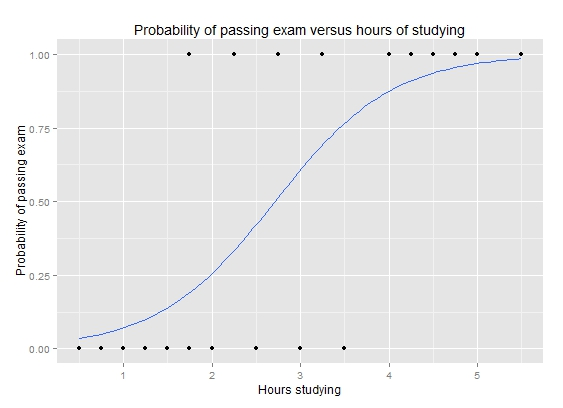
\includegraphics[width=0.7\textwidth]{img/Exam_pass_logistic_curve.jpeg}
    \caption{\label{fig:researchscope}By Michaelg2015 - Own work, CC BY-SA 4.0, https://commons.wikimedia.org/w/index.php?curid=42442194}
\end{figure}
\end{frame}
